\documentclass{article}
\usepackage[hmargin=1.5cm,vmargin=1.65cm]{geometry}
\usepackage{tikz} 

\begin{document}


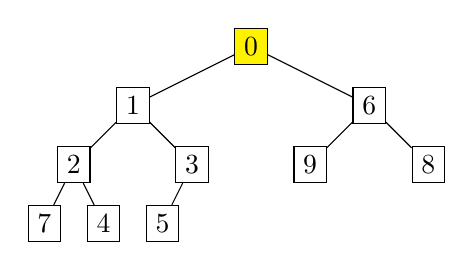
\begin{tikzpicture}[scale=0.5]
\tikzstyle{level 1}=[sibling distance=6.0cm]
\tikzstyle{level 2}=[sibling distance=3.0cm]
\tikzstyle{level 3}=[sibling distance=1.5cm]
\node[draw, fill=yellow] {0}
    child {node[draw] {1}
        child {node[draw] {2}
            child {node[draw] {7}}
            child {node[draw] {4}}
        }
        child {node[draw] {3}
            child {node[draw] {5}}
            child[fill=none] {edge from parent[draw=none]}
        }
    }
    child {node[draw] {6}
        child {node[draw] {9}}
        child {node[draw] {8}}
    };
\end{tikzpicture}
%
$\quad$
%
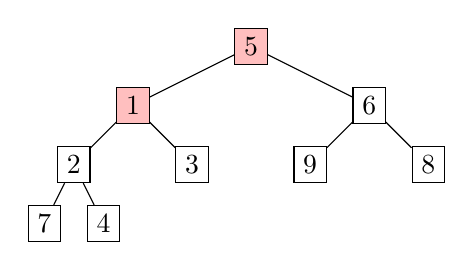
\begin{tikzpicture}[scale=0.5]
\tikzstyle{level 1}=[sibling distance=6.0cm]
\tikzstyle{level 2}=[sibling distance=3.0cm]
\tikzstyle{level 3}=[sibling distance=1.5cm]
\node[draw, fill=pink] {5}
    child {node[draw, fill=pink] {1}
        child {node[draw] {2}
            child {node[draw] {7}}
            child {node[draw] {4}}
        }
        child {node[draw] {3}}
    }
    child {node[draw] {6}
        child {node[draw] {9}}
        child {node[draw] {8}}
    };
\end{tikzpicture}
%
$\quad$
%
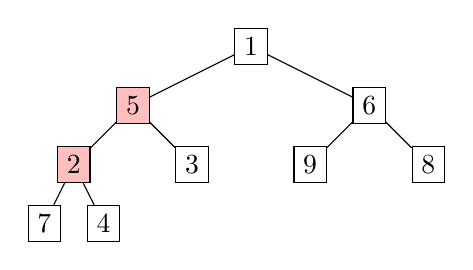
\begin{tikzpicture}[scale=0.5]
\tikzstyle{level 1}=[sibling distance=6.0cm]
\tikzstyle{level 2}=[sibling distance=3.0cm]
\tikzstyle{level 3}=[sibling distance=1.5cm]
\node[draw] {1}
    child {node[draw, fill=pink] {5}
        child {node[draw, fill=pink] {2}
            child {node[draw] {7}}
            child {node[draw] {4}}
        }
        child {node[draw] {3}}
    }
    child {node[draw] {6}
        child {node[draw] {9}}
        child {node[draw] {8}}
    };
\end{tikzpicture}

\vspace*{1cm}

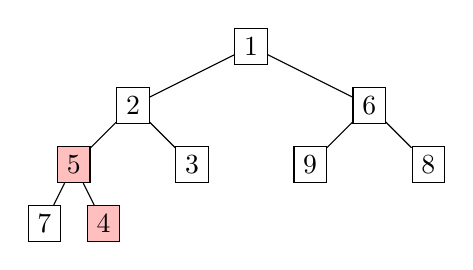
\begin{tikzpicture}[scale=0.5]
\tikzstyle{level 1}=[sibling distance=6.0cm]
\tikzstyle{level 2}=[sibling distance=3.0cm]
\tikzstyle{level 3}=[sibling distance=1.5cm]
\node[draw] {1}
    child {node[draw] {2}
        child {node[draw, fill=pink] {5}
            child {node[draw] {7}}
            child {node[draw, fill=pink] {4}}
        }
        child {node[draw] {3}}
    }
    child {node[draw] {6}
        child {node[draw] {9}}
        child {node[draw] {8}}
    };
\end{tikzpicture}
%
$\quad$
%
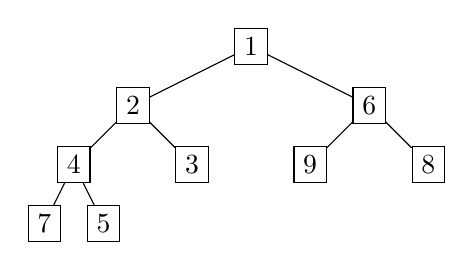
\begin{tikzpicture}[scale=0.5]
\tikzstyle{level 1}=[sibling distance=6.0cm]
\tikzstyle{level 2}=[sibling distance=3.0cm]
\tikzstyle{level 3}=[sibling distance=1.5cm]
\node[draw] {1}
    child {node[draw] {2}
        child {node[draw] {4}
            child {node[draw] {7}}
            child {node[draw] {5}}
        }
        child {node[draw] {3}}
    }
    child {node[draw] {6}
        child {node[draw] {9}}
        child {node[draw] {8}}
    };
\end{tikzpicture}


\end{document}  
